

\section{Spatial Label Smoothing}\label{spatial_smoothing}

The atmospheric variables within the ClimateNet dataset lack the sharp edges found in natural imagery. Physical phenomena like Tropical Cyclones and Atmospheric Rivers transition gradually into the background space. Rigid binary ground truth masks force the model into making definitive choices on ambiguous boundary pixels. This rigid penalty structure causes the model to memorize specific noise, leading to overfitting for the smaller TC class during later training epochs, as empirically observed. Applying a Gaussian blur to the ground truth masks before calculating the hybrid loss creates a continuous spatial gradient. This smooth gradient acts as a spatial regularizer that aligns more accurately with the physical reality of gradual pressure drop offs. Figures \ref{fig:blur_examples} illustrate the effect of label smoothing with varying kernel sizes and sigma values.


\begin{figure}[!h]
    \centering
    \makebox[\textwidth][c]{%
        \begin{minipage}{1.0\textwidth}
            \centering
            \begin{minipage}{0.48\textwidth}
                \centering
                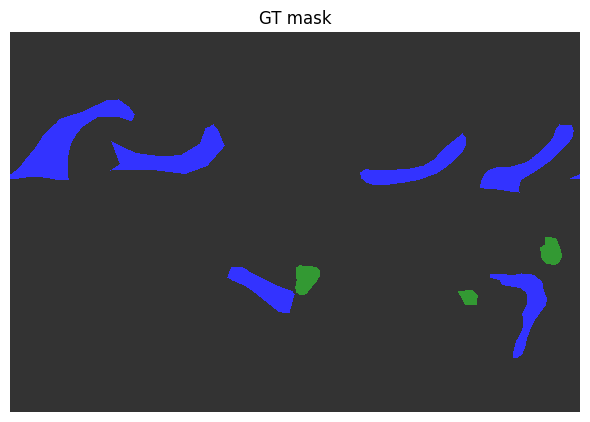
\includegraphics[width=1.05\textwidth]{graphics/approach/blur_0.png}
            \end{minipage}
            \hfill
            \begin{minipage}{0.48\textwidth}
                \centering
                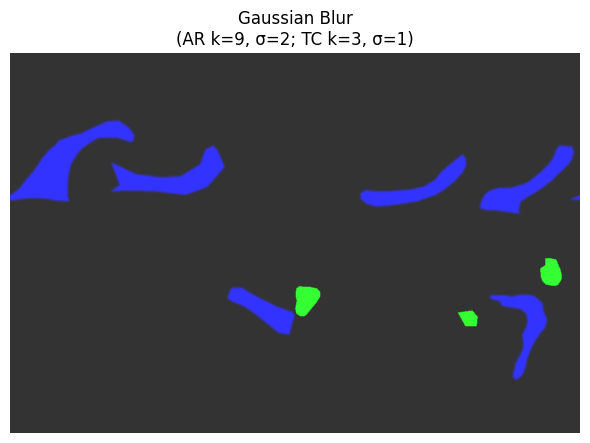
\includegraphics[width=1.05\textwidth]{graphics/approach/blur_1.png}
            \end{minipage}

            % \vspace{0.5cm}

            \begin{minipage}{0.48\textwidth}
                \centering
                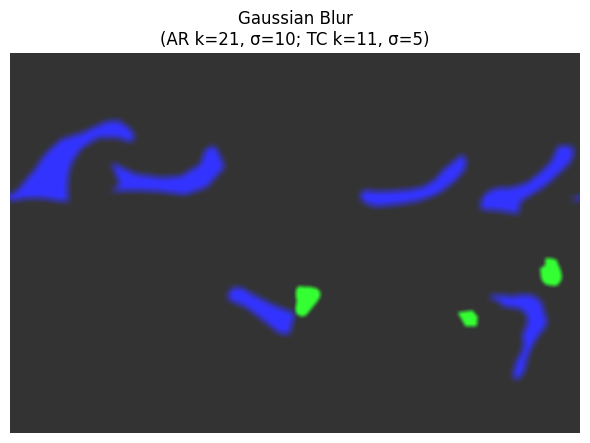
\includegraphics[width=1.05\textwidth]{graphics/approach/blur_2.png}
            \end{minipage}
            \hfill
            \begin{minipage}{0.48\textwidth}
                \centering
                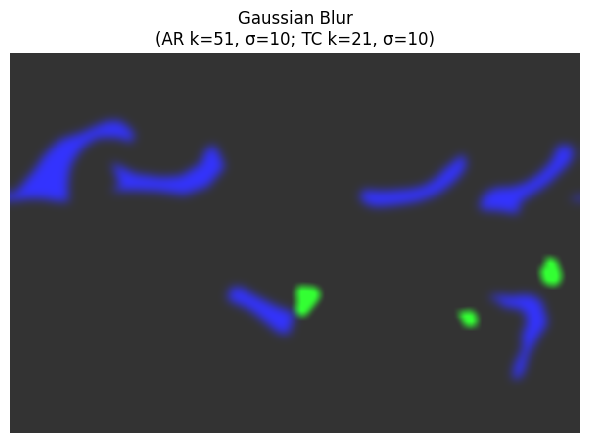
\includegraphics[width=1.05\textwidth]{graphics/approach/blur_3.png}
            \end{minipage}
        \end{minipage}
    }
    \caption{Example of label smoothing with different kernel sizes and sigma values.}
    \label{fig:blur_examples}
\end{figure}


Empirical tests confirm that applying a baseline spatial blur with a kernel size of 3 and sigma of 1.0 for Tropical Cyclones, alongside a kernel size of 9 and sigma of 2.0 for Atmospheric Rivers, successfully mitigates this overfitting behavior and significantly improves performance. Motivated by this success, we establish an independent grid search to identify the optimal blur configuration for each phenomenon. Because TCs and ARs differ drastically in scale, the search space is divided into two independent phases to isolate the effects of the smoothing parameters.

Table \ref{tab:smooth_search} summarizes the hyperparameter search space for the spatial label smoothing. During the search, when the parameters for one class are varied, the parameters for the other class are locked to their respective empirical baseline values to ensure an independent evaluation of the structural boundaries.

\begin{table}[h]
\centering
\begin{tabular}{lll}
Feature & Parameter & Search Values \\
\hline
TC & Kernel Size ($k\_{tc}$) & 3, 11, 21 \\
TC & Sigma ($\sigma\_{tc}$) & 1, 5, 10 \\
AR & Kernel Size ($k\_{ar}$) & 9, 21, 51 \\
AR & Sigma ($\sigma\_{ar}$) & 2, 10, 20 \\
\hline
\end{tabular}
\caption{Hyperparameter search space for spatial label smoothing.}
\label{tab:smooth_search}
\end{table}